\chapter{GPGPU-Based Implementation of a finite difference algorithm}

\section{Introduction}

Now that we have given an introduction to the theoretical and numerical aspects of the thesis,
the object of this section is to give an overview of the implemenation of an algorithm using finite difference schemes.
The source code used for the computations is based on an existing version from [A.Tilgner].
It was furthermore optimized  and extended by the immersed boundary methods, which will be explained in more detail in chapter (5.).
Especially in this context we will introduce some aspects of GPGPU\footnote{General Purpose Computation on Graphics Processing Unit - Allg.  Bezeichung für Allzweck-Berechnungen auf Grafikprozessoren}-Computing
with the CUDA \footnote{Computing Uniform Device Architecture} architecture.
For the computations the  Tesla C1060 and Tesla K20m GPUs by NVIDIA were used, the complete system configurations can be looked up at (AX.X).

\section{GPGPU-Computing with CUDA}

CUDA is an architecture developed by NVIDIA to enable an easy approach to the Implementation of GPGPU-based algorithms.
The underlying idea is to hide the complexity of the hardware under a more high oriented and generalized software abstraction layer.
This is done by introducing some additional programming language extensions i.e. in c/c++\footnote{WIR BENUTZEN C/C++ /PYTHON ETC},
furthermore it is necessary to use a CUDA suited compiler like NVCC.

For the development of a highly efficient working algorithm, we need to keep in mind the memory architecture used in CUDA, as
exemplary shown in figure (X).

\begin{figure}[!tbp]
  \centering
  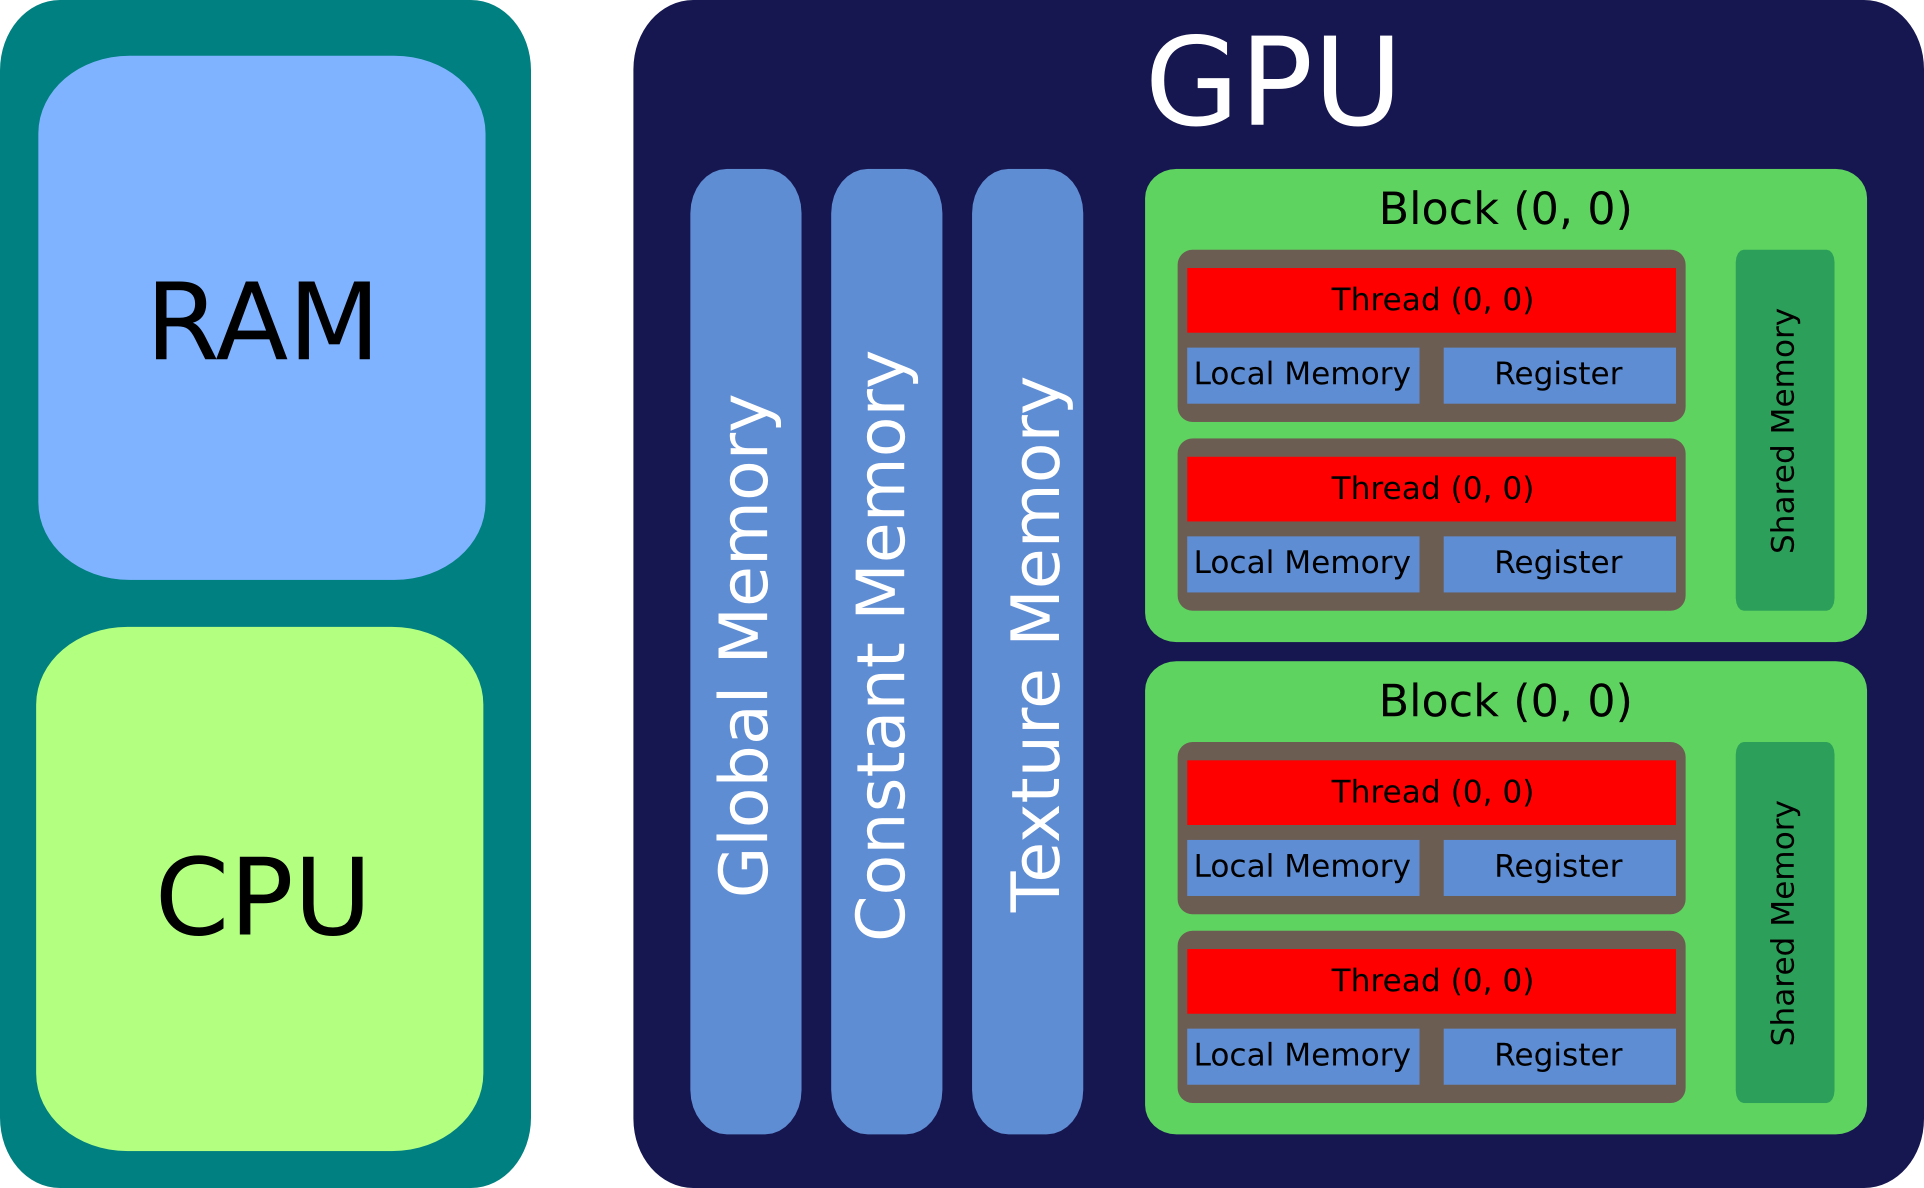
\includegraphics[width=0.8\textwidth]{gfx/cuda/gpu.png}\label{fig:gpu_arch}
  \caption{Speicherlayout einer Nvidia-GPU}
\end{figure}

It should be noted that this layout is not directly related to the underlying hardware.
The gpu is connected by the pci-express x16 bus to CPU and RAM of the Computer.
There is some kind of main memory on the gpu which is divided in Global Memory, Constant Memory and Texture Memory.

- what is a block
    -streaming machine with cuda cores
    - shared memory
    -

- what is a thread
- streaming processor


-z.b. ist der local memory auf der karte im global memory speicherbereich

- lese paper / präsi zur optimierung
- geschwindigkeiten
- shared vs global etc

\subsection{CUDA syntax example}

-grid layout function call
-blocks
-threadidx etc
-memcpy

\section{Algorithmus}
-oder so ?
-erläuterung  implementierung
-speicherverwaltung

\section{Optimierung}
- coalesceded
- bank conflicts?
- teilvolumen nicht rechnen

\section{Validierung}
- beispiel rayleigh benard system
- masa
- vgl o2 vs o4 masa cube
- bifurcation


\newpage

